\chapter{Fundamentación Teórica. Electrónica y Computación}
\label{teoria}
La teoría que se puede aplicar a los componentes del sistema a implementar en este trabajo pueden ser bastante complejos. Sin embargo, no es necesario un análisis profundo en un sistema de control de panel solar con una carga resistiva. Por lo que se explica solo lo necesario para el comprender del funcionamiento y razón sobre la elección de los componentes en un sistema real.
\section{Electrónica de Potencia}
Para realizar un control de potencia en continua, la electrónica emplea componentes semiconductores (Figura \ref{fig:semicon}) en circuitos llamados Conversores DC-DC (Figura \ref{fig:topologiassimples}).
\begin{figure}[H]
    \centering
    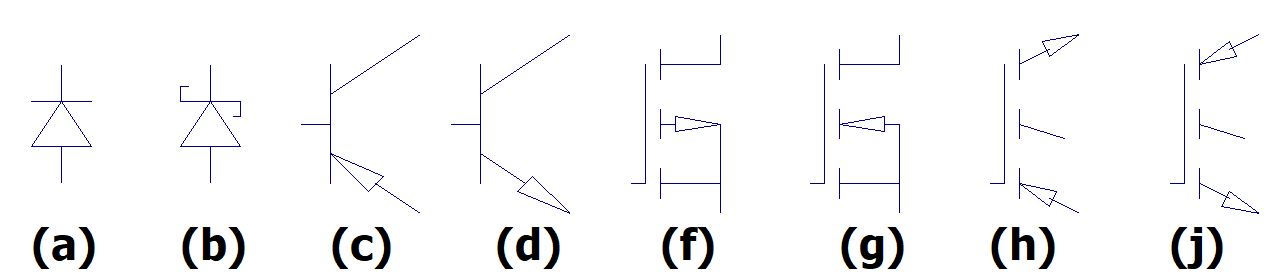
\includegraphics[width=\linewidth]{imagenes/semiconductores.png}
    \caption{Interruptores unipolares de acción simple: (a) Diodo simple, (b) Diodo Schottkey, (c) Transistor BJT tipo P y (d) tipo N, (f) Mosfet tipo P y (g) N, (h) IGBT tipo P y (j) N}
    \label{fig:semicon}
\end{figure}

\begin{figure}[H]
    \centering
    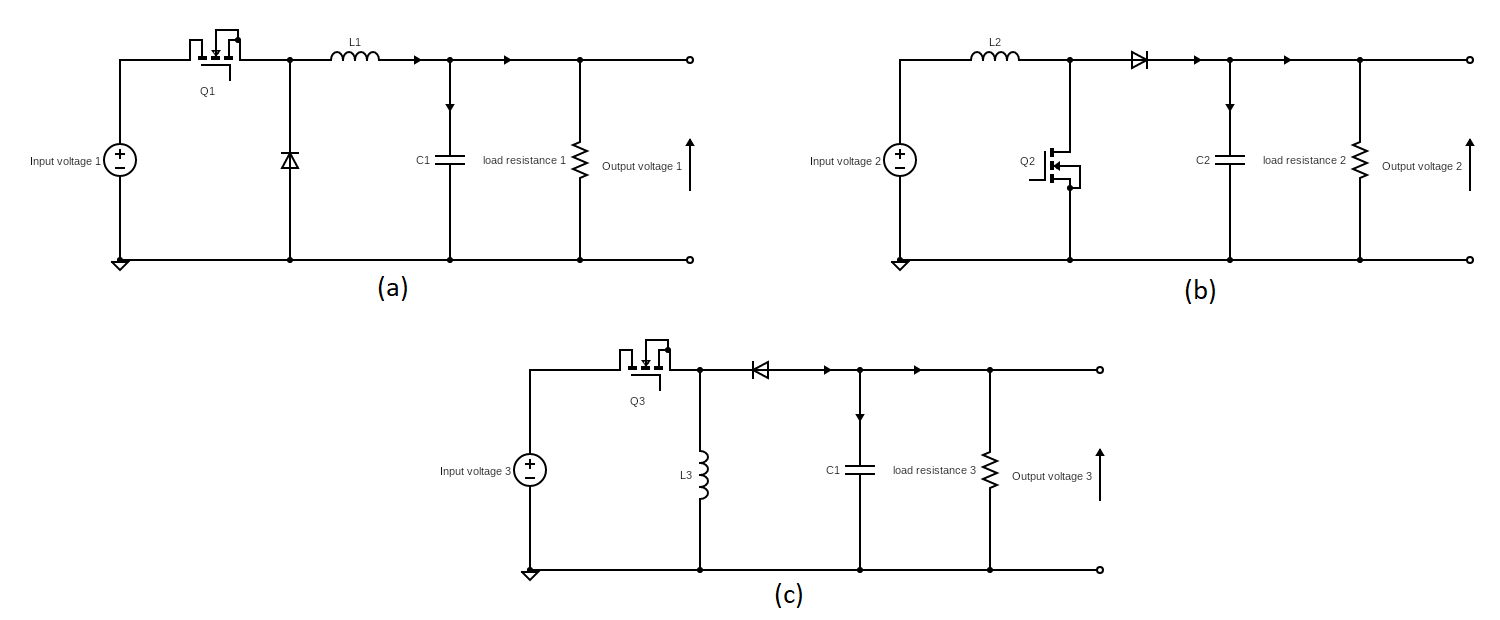
\includegraphics[width=\linewidth]{imagenes/simpletopologies.png}
    \caption{Conversores DC-DC no aislados: (a) Buck, (b) Boost, (c) Buck-Boost}
    \label{fig:topologiassimples}
\end{figure}
Obviamente, no son los únicos circuitos conversores DC-DC existentes los ilustrados en la figura \ref{fig:topologiassimples}, sino los mas simples de implementar matemática y físicamente hablando. El desarrollo de este tipo de conversores continua actualmente \cite{power}, pero la implementación de estos se escapa del alcance del presente trabajo.\par La elección de que topología utilizar de la Figura \ref{fig:topologiassimples} dependerá de la respuesta deseada del sistema.
\subsection{Semiconductores}
Los dispositivos semiconductores en potencia se comportan como interruptores unipolares de acción simple, y dependiendo de los parámetros deseables en la implementación es la elección de uno sobre otro. 
\subsubsection{Diodo}
El diodo es un semiconductor de materiales n y p 
El diodo entra en estado de polarización al conectarle en los contactos una tensión. Dependiendo de la tensión es una polarización directa o inversa.\par \par Unas de las mayores ventajas de los diodos Schottky es su rápida velocidad de conmutación y una baja caída de voltaje al estar polarizado en modo directo. Incluso el tiempo transitorio de recuperación inversa no es importante. Sin embargo, pocos dispositivos comerciales superan una tensión de ruptura de 100V. Por lo que son preferibles ante sistemas de bajo voltaje (45V o menos). Otro problema es que la corriente de fuga mayor que la de un diodo de silicio comparable \cite{power}.\par 
\subsubsection{MOSFET}
Mosfet rapido veloz
\subsection{Conversores DC-DC}

    
\subsubsection{Buck Síncrono}
\begin{equation} \label{potin}
	P_{in} = {V_{in} \times  I_{in}}
	\end{equation}
\begin{equation} \label{potout}
	 P_{out} = {V_{out} \times  I_{out}} 
\end{equation}
\begin{equation} \label{potineqpotout}
	 P_{in}\times\eta = P_{out}
\end{equation}
\begin{equation} \label{potinaproxpotout}
	 P_{in}\approx P_{out}
\end{equation}
\begin{equation} \label{voutvioniiniout}
	 {V_{in} \times  I_{in}} = {V_{out} \times  I_{out}} 
\end{equation}
\begin{equation} \label{vinDvout}
	 {V_{in} \times  D} = {V_{out} } 
\end{equation}
\begin{equation} \label{iinioutd}
	{ I_{in} \times \frac{1}{D}} = {I_{out}} 
\end{equation}
\begin{equation} \label{limitesded}
	{0\leq D \leq 1}
\end{equation}
\begin{equation} \label{rinprima}
	{ R_{in}'} = {\frac{V_{in}}{I_{in}}} 
\end{equation}
\begin{equation} \label{routprima}
	{ R_{out}} = {\frac{V_{out}}{I_{out}}} 
\end{equation}
\begin{equation} \label{rinandrouteq}
	{ R_{in}'\times I_{in} \times I_{in}} = {R_{out}\times I_{out} \times I_{out}} 
\end{equation}
\begin{equation} \label{rinroutsquare}
	{ R_{in}'\times I_{in}^2} = {R_{out}\times I_{out}^2} 
\end{equation}
\begin{equation} \label{rinroutsquareoniinonesquare}
	{ R_{in}'\times I_{in}^2} = {R_{out}\times (\frac{I_{in}}{D})^2} 
\end{equation}
\begin{equation} \label{rinroutsquareoniin}
	{ R_{in}'\times I_{in}^2} = {R_{out}\times I_{in}^2 \times \frac{1}{D^2}} 
\end{equation}
\begin{equation} \label{rinroutalmostfinal}
	{ R_{in}'} = {R_{out}\times \frac{1}{D^2}} 
\end{equation}
\begin{equation} \label{rinroutfinal}
	{D} = {\sqrt{\frac{R_{out}}{R_{in}'}}} 
\end{equation}
\begin{equation} \label{routlessrin}
	R_{out}<R_{in}'
\end{equation}
\begin{equation} \label{rinbaseonrout}
	R_{in}'={\frac{R_{out}}{D^2}}
\end{equation}
\begin{equation} \label{frecuenciadetanke}
	f_c={\frac{1}{2\times \pi \times \sqrt{L\times C}}}
\end{equation}
\begin{equation} \label{fcmenorfs}
	f_c<<f_s
\end{equation}
\begin{equation} \label{fcmayorfs}
	f_c>>f_s
\end{equation}
\begin{equation} \label{deltail}
	\Delta I_L={\frac{V_{in}\times D \times(1-D)}{f_s\times L}}
\end{equation}
\begin{equation} \label{deltavc}
	\Delta V_c={\frac{V_{in}\times D \times(1-D)}{8\times f_s^2\times L \times C}}
\end{equation}
\begin{equation} \label{calculodeinductancia}
	L={\frac{V_{out} \times(1-D)}{f_s\times \Delta I_L}}
\end{equation}
\begin{equation} \label{calculodecapacitancia}
	C={\frac{\Delta I_L}{8\times f_s\times \Delta V_c}}
\end{equation}
\begin{equation} \label{riplevout}
	{\frac{\Delta V_out}{V_out}}={\frac{\Delta I_L}{8\times f_s\times \Delta V_c}}
\end{equation}
\begin{figure}[H]
    \centering
    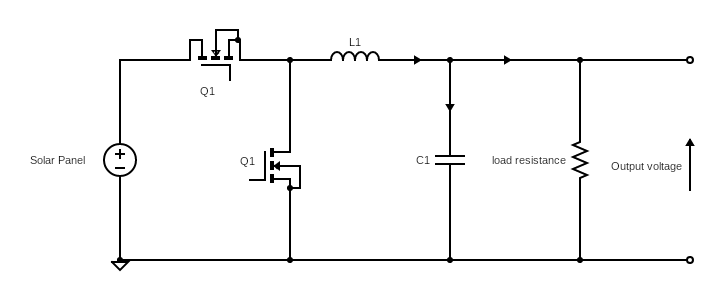
\includegraphics[width=1\linewidth,frame]{imagenes/syncbuck.png}
    \caption{Circuito de conversor Buck síncrono}
    \label{fig:circuito_final}
\end{figure}
\section{Paneles Solares}

\subsection{MPPT}

\subsection{Computación de MPPT}
El control en conversores DC-DC se da con una retroalimentación de tensión o corriente\cite{fundamental}, utilizando un circuito analógico generalmente para producir una tensión o corriente de salida estática. Sin embargo, para el control de sistemas fotovoltaicos, se emplea un control dinámico para obtener la máxima potencia, siendo este posible analógicamente en algunos casos, o dependientes de un sistema computacional. \par Los algoritmos de MPPT siguen evolucionando\cite{power}, sin embargo, se estudia el método básico de P\&O juntos con unas modificaciones.
\section{ESP32}
\subsection{MCPWM}
